\chapter{EEG/ERP Portal}
\label{chap:eegPortal}

This chapter describes the motivation behind the creation of the EEG/ERP Portal. Crucial technologies and frameworks that have been used in development of the EEG/ERP Portal are also described.

\section{About EEG/ERP Portal}

The EEG/ERP Portal (Figure \ref{fig:eegPortal}) is a web-based application which serves to neuroinformatics researchers as a means of managing, sharing and evaluating measured data. The application also comprises advanced features designed specifically for the needs of the EEG/ERP researchers, such as tools for manipulation with EEG signals.


\begin{figure}[h!]
	\centering
		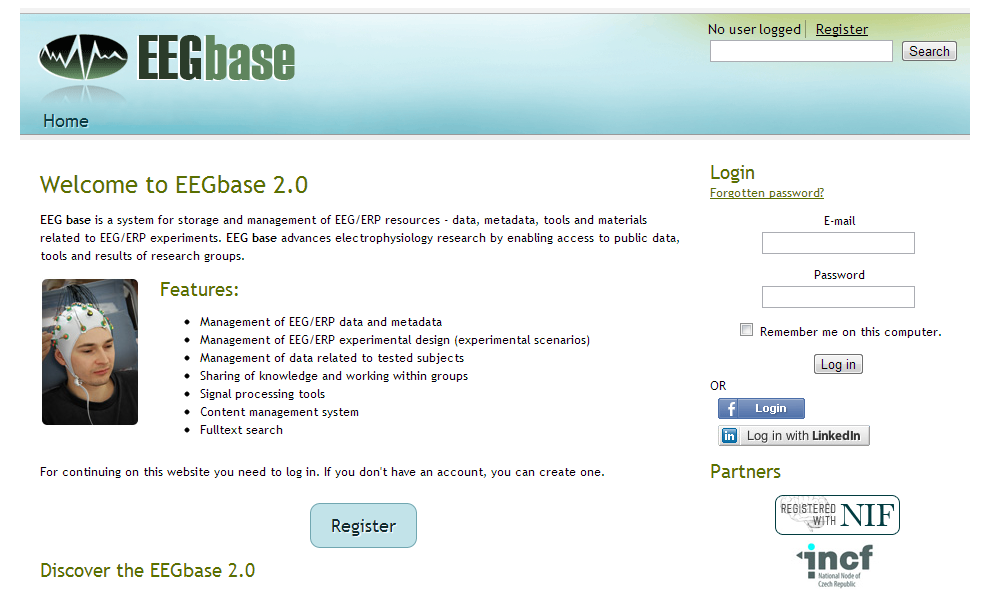
\includegraphics[width=1.00\textwidth]{figures/eegPortal.png}
	\caption{EEG/ERP Portal Welcome Page.}
	\label{fig:eegPortal}
\end{figure}

% V nasledujicich oddilech budou ve zkratce popsany technologie, ktere Hibernate pouziva, a budou popsany nektere aspekty, se kterymi se potyka text v prakticke casti prace

\section{Hibernate}

% Strucne popsat, k cemu je Hibernate a jaky vyuziti ma v portalu. Mozna taky vlozit nejaky schema (z BP?)
Hibernate \cite{Hibernate:Home} is an open-source object-relational mapping framework, whose purpose is to facilitate storage and retrieval of Java domain objects. It is used in the EEG/ERP Portal to map its data model to the object model and vice versa.


%Since the practical part of the thesis will be partially devoted to , it is necessary to explain Hibernate loading strategies first.

%is a high-performance, mature object-relational mapping (ORM) library. As a non-intrusive ORM solution, Hibernate provides object query APIs for plain old Java object (POJO) persistence model classes and automatic data bindings between the object and relational representations of persistence data. In essence, it lets you focus on domain model-oriented programming. 


% HOTOVO

\subsection{Hibernate loading strategies}
% zminit, ze Hibernate ruzne nahrava objekty

% https://community.jboss.org/wiki/LazyInitializationExceptionOvercome?_sscc=t

Hibernate provides two strategies of fetching data from the database to their object representations. 
As an analogy to database relationships, the POJO objects can maintain associations to other objects. 
The strategies differ in the way they treat these object associations, both having their advantages and disadvantages. 

The first possible way is to load all associated object collections at the same time when the database record corresponding to the object is fetched. 
This is called \textit{eager loading}. 
The second way is to return only the data belonging directly to the object and not to fetch the collections until they are required to be fetched. 
This approach is known as \textit{lazy loading}. 

Lazy loading is generally considered a preferred way in most of the applications.
The main reason behind this is performance effectiveness.
When a certain POJO object (actually the underlying table record) is accessed, it is sufficient for most of the use cases to fetch only the fields of primitive types, because associated collections are not needed. 
By using lazy loading in such scenarios, many unnecessary join and select operations are often avoided. 
In the end, the operation savings reflect both in lower time and memory costs which results in faster application responses. 

On the contrary, overusing eager loading can considerably slow down the application and may lead to the \textit{n+1 selects problem} described e.g. in \cite{HibernateInAction:2004}.	
However, there are many reasonable situations when all associated object data have to be always available. 
As an example, one can imagine a requirement to always display writers together with all the books they have written. 
Then it is completely legitimate to apply eager loading to load the books for each of their authors because of the certainty specified by the requirement.

There are also cases when it is desired to load otherwise lazily initialized collections eagerly.
Hibernate also allows enforcing temporary eager loading.

To understand how lazy loading works in Hibernate, it is important to briefly explain the dynamic proxy pattern. 

\subsubsection{Dynamic proxy}

Hibernate uses dynamic proxies to implement lazy loading of object properties. 
The \textit{``Design Patterns''} book written by \textit{Gang of Four} (GOF) \cite{GOF:DesignPatterns} describes the proxy pattern the following way:

\begin{quote}		
\textit{``Allows for object level access control by acting as a pass through entity or a placeholder object.''}
\end{quote}


\begin{figure}[h]
	\centering
		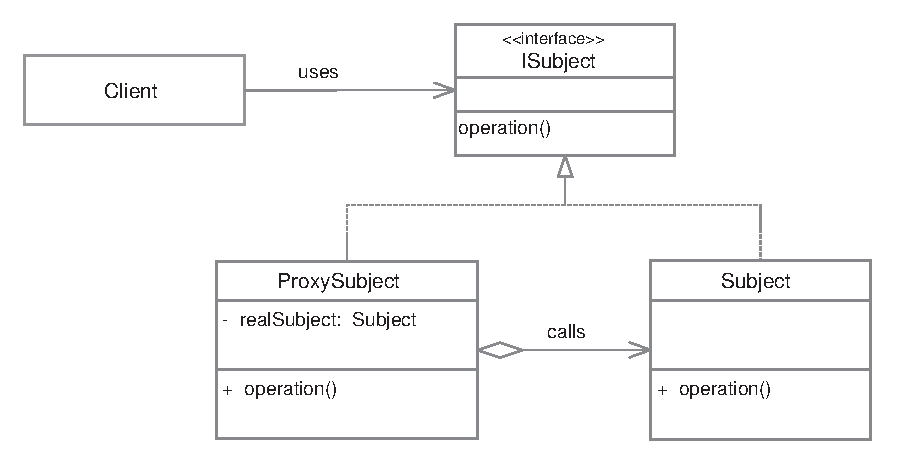
\includegraphics[width=0.7\textwidth]{figures/proxy.eps}
	\caption{Proxy Design Pattern.}
	\label{fig:proxy}
\end{figure}


When an object is required to be loaded, some of its object properties are not actually fetched from the database. Instead, they are represented by their corresponding proxy objects. 
The proxy object is usually referred to as \textit{stub} and does not hold any actual information. 
Its only ability is to call the real object it represents. The UML diagram depicted in figure \ref{fig:proxy} helps visualize the whole mechanism.
Since these stub objects are in case of Hibernate created dynamically at runtime by using the bytecode libraries \textit{javassist} or \textit{CGLIB}, we talk about dynamic proxies. 

\section{Spring Framework}

% Popsat strucne, jak funguje, jak se vyuziva
The Spring Framework \cite{SpringFramework:Home} facilitates creating Java-based enterprise applications. It applies a principle called \textit{dependency injection} which helps make the classes loosely coupled. The idea of this principle is to let the framework do all necessary wiring of objects, so that the objects can focus on their core responsibilities. By reducing dependencies among application components, the code becomes more testable and reusable. A thorough explanation of the dependency injection principle can be found for example in Martin Fowler's infamous article \cite{Fowler:DI}. 

\subsection{Spring Social}

Spring Social is one of the Spring Framework extensions that was created to enable easier connection of Spring-based applications with Software-as-a-Service (SaaS) providers, like Facebook, LinkedIn, Twitter and others.
The EEG/ERP Portal uses Spring Social to interact with LinkedIn. % teorie -> premistit
Spring Social offers a bunch of methods which wrap the existing LinkedIn REST API calls. % teorie -> premistit 

\subsubsection{LinkedIn REST API} 
% Co to je, k cemu to je,
% http://www.youtube.com/watch?v=xy8jfKTOiuc
LinkedIn provides REST API to access various information. 
\textit{Representational State Transfer} (REST) is pragmatically defined in \cite{REST:Introduction} as \textit{``a set of principles that define how Web standards, such as HTTP and URIs, are supposed to be used''}.
REST takes the advantage of the HTTP protocol to describe the action that should be performed on a given resource.
Resource is an entity that can be identified by URL.
Internal domain model of LinkedIn, which includes entities like people, companies and jobs, is mapped to REST resources. 

Required information one wishes to obtain can be specified by URI parameters in the JSON format. Examples of its usage are contained in the practical part of the thesis in Chapter \ref{chap:implementation}.


\section{Wicket}

% Popsal v par vetach a uvest, proc se na nej preslo.
Wicket \cite{Wicket:Home} is a component-based framework for creating user interface of web applications. 
The EEG/ERP Portal's presentation layer is being developed in Wicket by the time of writing this thesis. 
In the case of the EEG/ERP Portal, it is a replacement of JSP pages and Spring MVC. 
This decision was made due to clearer separation of application logic and markup which, in effect, leads to more readable and maintainable code.

A web page created by using the Wicket framework consists of a HTML file that determines the page appearance, and a paired Wicket \texttt{WebPage} class instance that contains a component hierarchy. % uses the provided Wicket components or builds upon them.
The binding of HTML files and their relevant Java classes is done by specifying component identifiers. In case of an HTML page, a value set to the special \texttt{wicket:id} tag attribute identifies a Wicket component. The same value of the component name must be then specified in the matching component in Java code.
